\documentclass[a4paper]{scrartcl}%{{{
\usepackage{float}
\usepackage{tikz}
\usetikzlibrary{arrows,automata}
\usepackage{pgf}
\usepackage[utf8]{inputenc} % this is needed for umlauts
\usepackage[ngerman]{babel} % this is needed for umlauts
\usepackage[T1]{fontenc}    % this is needed for correct output of umlauts in pd
\usepackage{amssymb}
\usepackage{amsmath}
\usepackage{mathabx}
\usepackage{mathrsfs}
\usepackage{dsfont}
\usepackage{wasysym}
\usepackage{graphicx}
\usepackage{fancyhdr}
\usepackage{lastpage}
\usepackage{imakeidx}
\setlength{\parskip}{\medskipamount}
\setlength{\parindent}{0pt}
\usepackage{enumitem}
\usepackage{hyperref}
\usepackage{verbatim}

%%%%%%%%%%%%%%%%%%%%%%%%
% Kopf- und Fusszeilen %
%%%%%%%%%%%%%%%%%%%%%%%%
\pagestyle{fancy}
\lhead{
        Maximilian Roth
}
\chead{Logik-Tutorat Lösungen Blatt 11\\}
\rhead{
    \begin{tabular}{rr}
        \today{} \\
        Seite \thepage{} von \pageref{LastPage}
    \end{tabular}
}
\lfoot{}
\cfoot{}
\rfoot{} 

%%%%%%%%%%%%%%%%%%%%%%%%
% Anfang des Dokuments %
%%%%%%%%%%%%%%%%%%%%%%%%%
\begin{document}
\section*{Disclaimer}
\label{sec:disclaimer}
Auch in diesem Dokument können sich Fehler befinden!\\
Sie sind nicht die Musterlösung der Aufgaben, sondern selbst erstellte Lösungen.\\

Als generelle Lektüre kann ich nur das Skript von Markus Junker aus dem WS 17/18 empfehlen:\\
\url{http://home.mathematik.uni-freiburg.de/junker/skripte/InfoLogik.pdf}\\
Hier ist vieles sehr genau und verständlich erklärt.
%}}}
\section*{}%{{{
\label{sec:aufgabe_1}

    \begin{figure}[H]
        \includegraphics[scale=0.3]{./A-1.png}
        \label{fig:}
    \end{figure}

    \begin{itemize}
        \item a)\\
            Genau wie \textcircled{1} a) auf Blatt 10. 
        \item b)\\
            Wir definieren folgendes g:\\
            $g(\bar{x}, y) =\\
            g(\bar{x}, y \dotdiv 1) + (\sum_{i \leq y \dotdiv 1}(f(\bar{x}, i) \neq 0) = y)$\\
            \\
            Wir sehen, dass dies gerade die gewünschte Fkt. ist.\\
            \begin{itemize}
                \item Fall 1: $g(\bar{x},y)$ mit y nicht das Minimum\\
                    $\Rightarrow \exists i<y: f(\bar{x}, i) = 0 \Rightarrow \sum_{i \leq y \dotdiv 1} \neq y$\\
                    Damit fallt also der zweite Term weg und es gilt:\\
                    \\$g(\bar{x},y) = g(\bar{x},y\dotdiv 1)$\\
                \item Fall 2: $g(\bar{x}, y)$ mit y Minimum\\
                    $\sum_{i \leq y \dotdiv 1} = y \text{ und } g(\bar{x},y\dotdiv 1) = y \dotdiv 1$, da wahr für alle kleineren i < y.\\
                    $\Rightarrow g(\bar{x},y) = y$\\
            \end{itemize}
            Da =, $\sum$ und $\neq_0$ primitiv rekursiv sind ist auch g (primitiv) rekursiv.\\
    \end{itemize}%}}}

\newpage

\section*{}%{{{
\label{sec:aufgabe_2}

    \begin{figure}[H]
        \includegraphics[scale=0.3]{./A-2.png}
        \label{fig:}
    \end{figure}

    \begin{itemize}
        \item a)\\
            \underline{ZZ:} Im(f) ist rekursiv.\\
            Um dies zu zeigen müssen wir zeigen, dass seine charakteristische Funktion rekursiv ist.\\
            \begin{itemize}
                \item Fall 1: Im(f) ist endlich:\\
                    Dann ist Im(f) rekursiv, da jede endliche Teilmenge von $ \mathds{N}^n$ rekursiv ist.\\
                \item Fall 2: Im(f) ist unendlich:\\
                    Damit muss f ewig lang wachsen (monoton steigend) und hat folgende Form (Beispiel):\\
                    \begin{figure}[H]
                        \centering
                        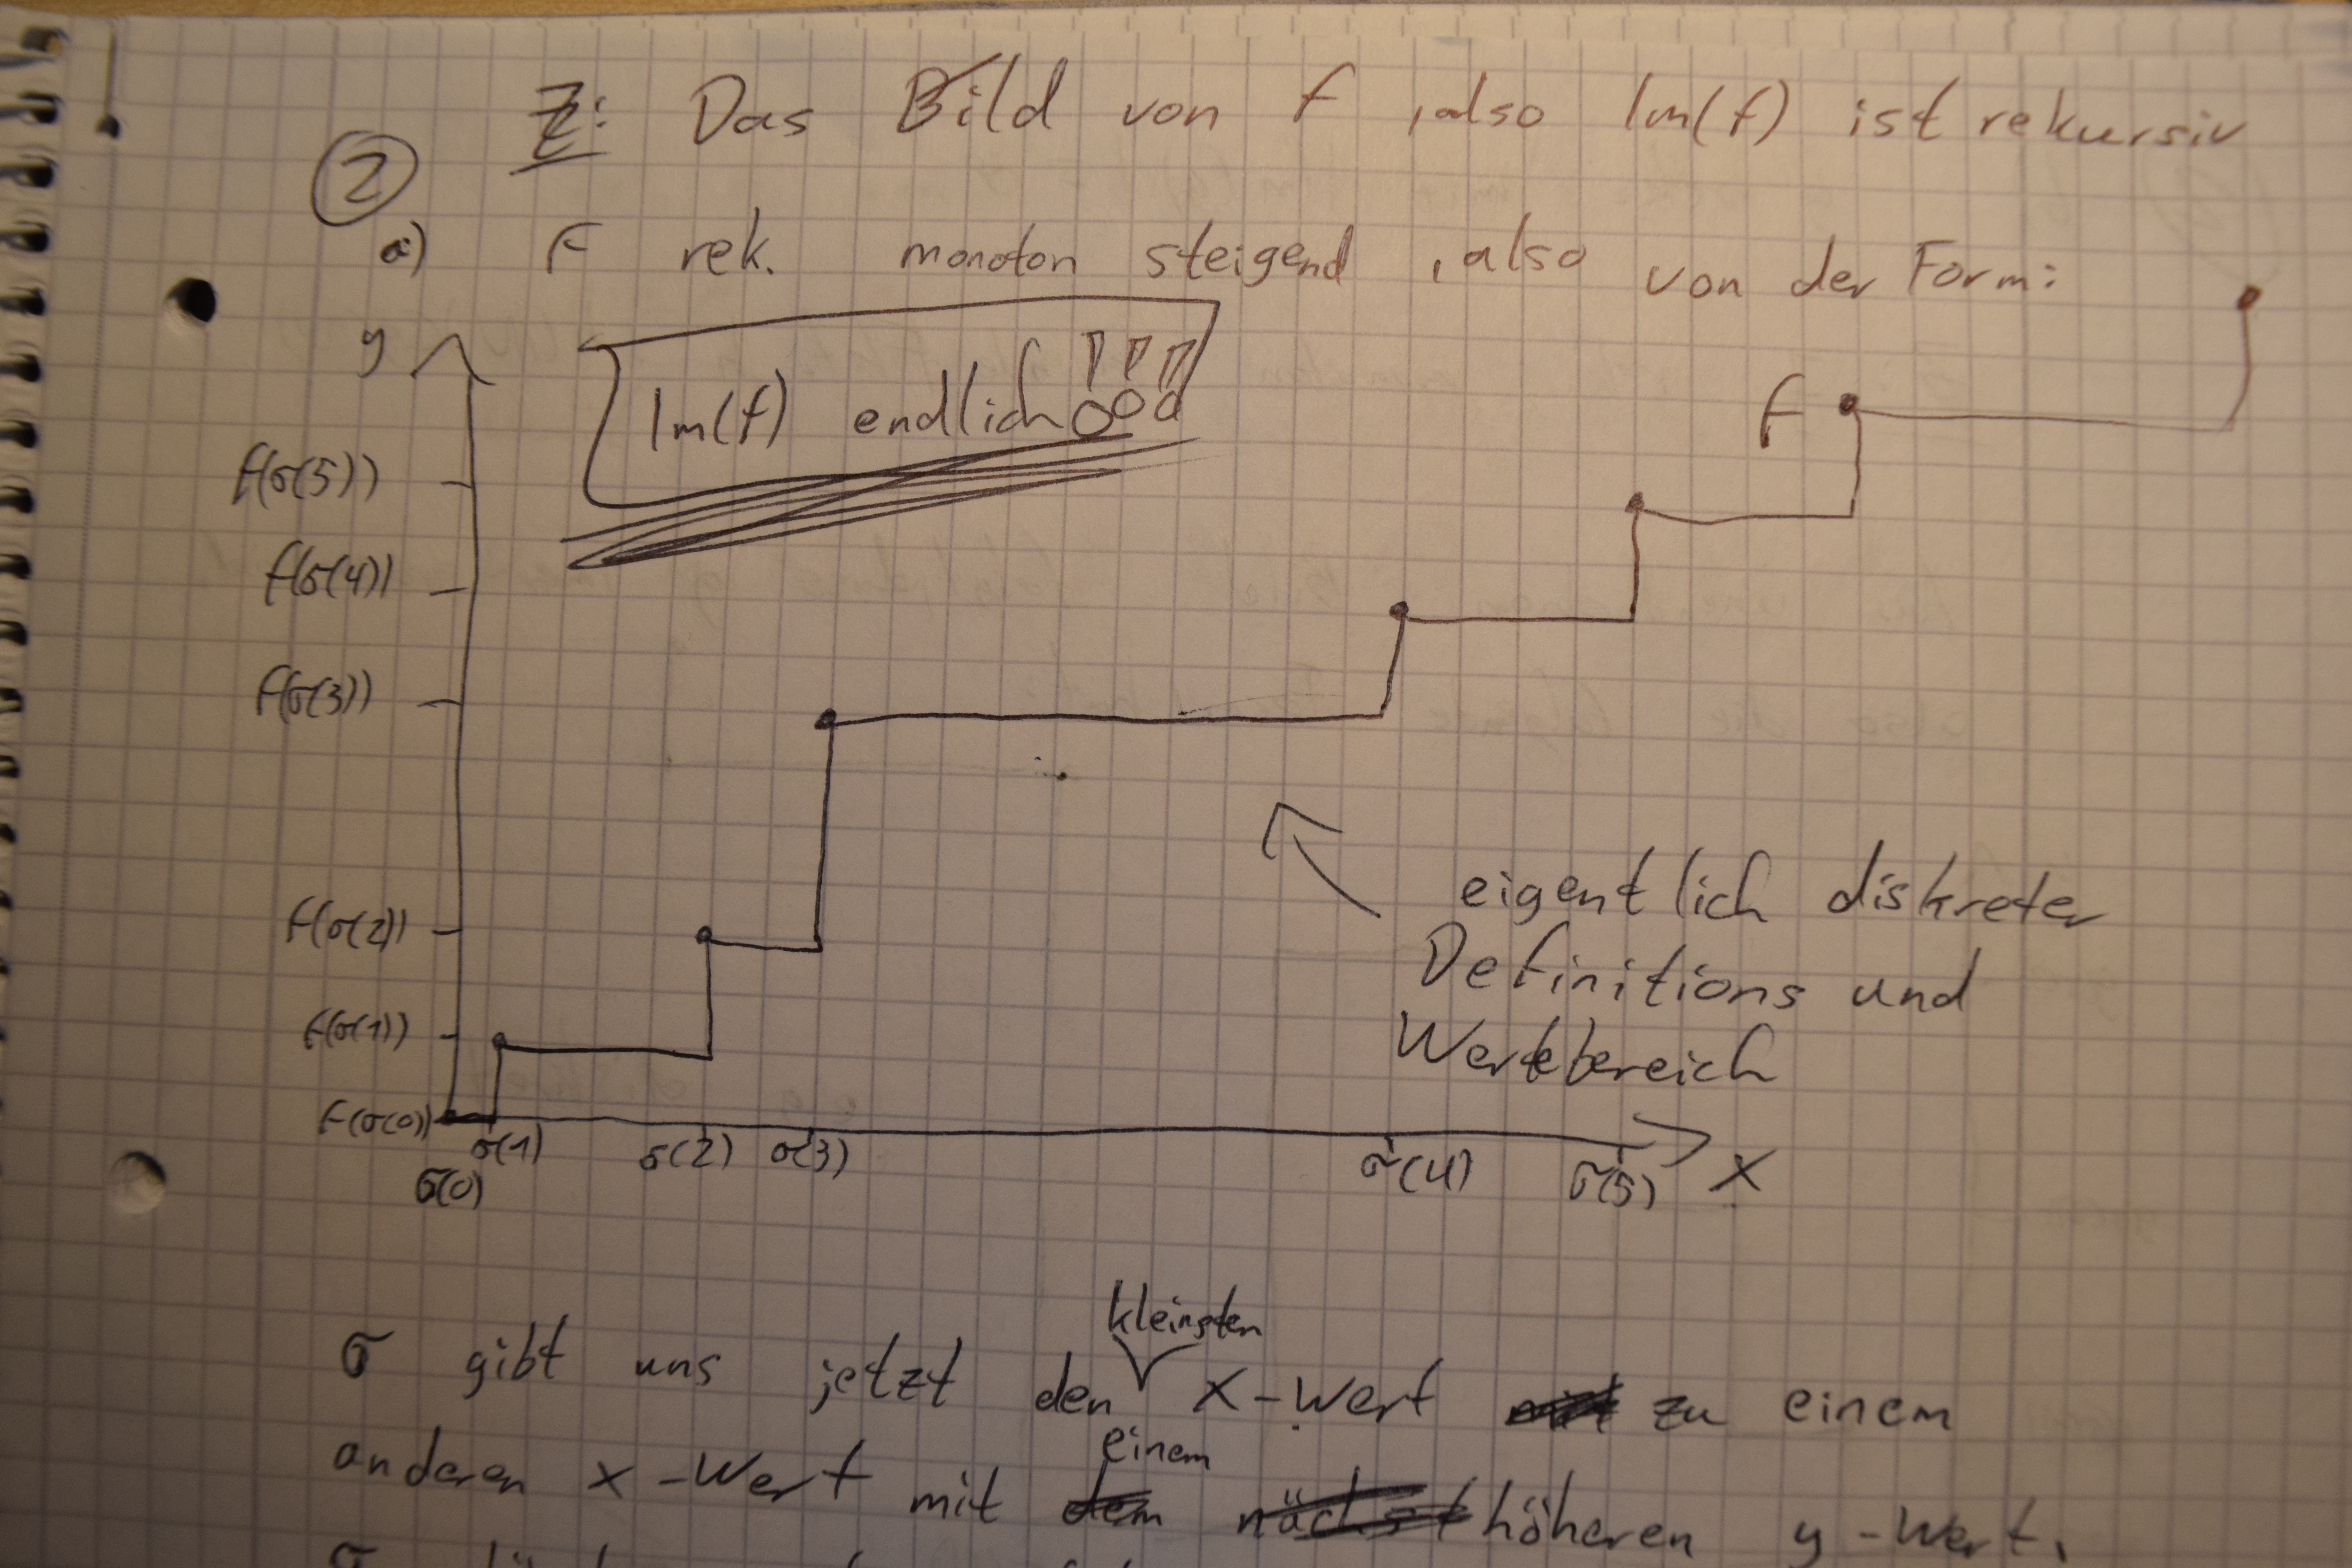
\includegraphics[scale=0.17]{./DSC_0585.JPG}
                        \label{fig:./DSC_0585}
                    \end{figure}

                    Es kann also das selbe Bildelement beliebig oft hintereinanderkommen (solange endlich).\\
                    Das macht es schwer eine rekursive Fkt. zu definieren.\\
                    \\Wir lösen dieses Problem mit einer Hilfsfunktion h, die das gleiche Bild hat, aber streng monoton steigt.\\
                    Das heißt h soll die Plateaus von f auslassen und nur die x-Werte betrachten, die einen größeren y-Wert haben, als ihr vorgänger.\\
                    \\Um diese x-Werte zu finden nutzen wir $\sigma$:\\
                    $\sigma(0) = 0$, da der erste Wert der kleinste des Bildes sein muss (monoton steigend).\\
                    $\sigma(n+1) = \mu m (f(\sigma(n))< f(m))$\\
                    \\Die $\mu$-Rekursion sucht genau den kleinsten x-Wert m mit höherem y-Wert f(m), als der aktuelle Punkt n (der den y-Wert f(n) hat).\\
                    \\Sei nun $h = f \circ \sigma$, dann ist h rekursiv und hat die Form:\\
                    \begin{figure}[H]
                        \centering
                        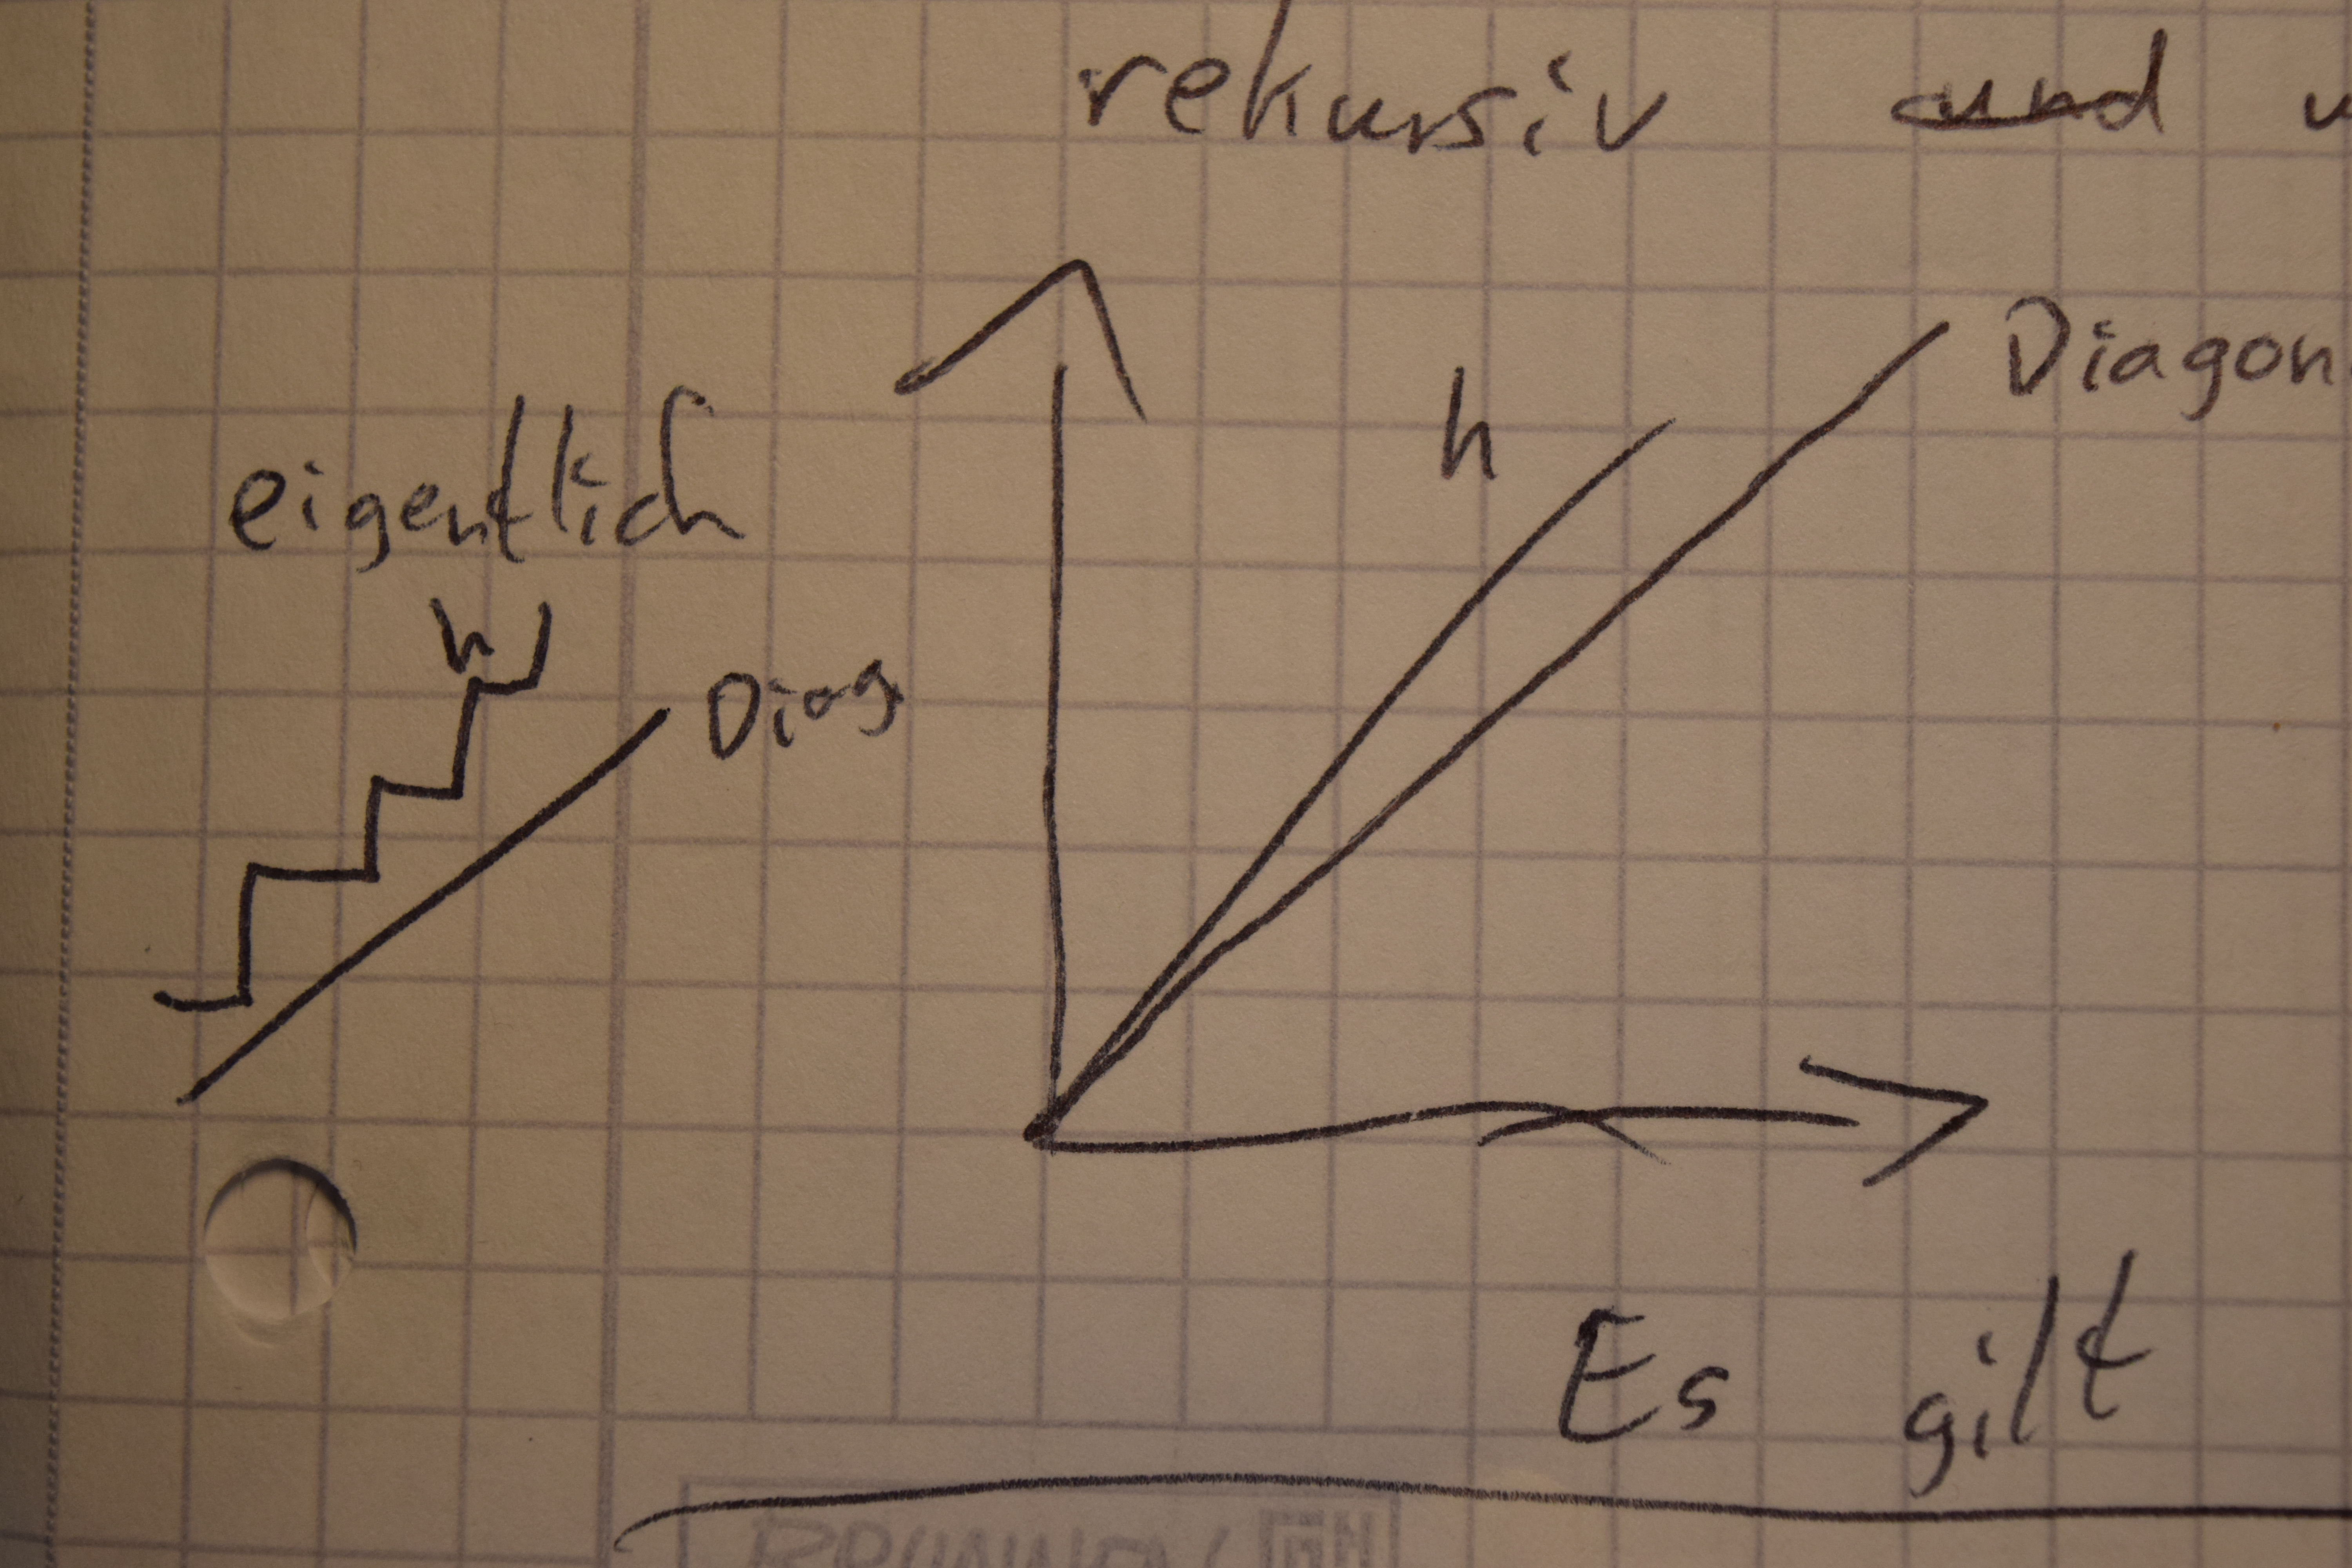
\includegraphics[scale=0.17]{./DSC_0586.JPG}
                        \label{fig:./DSC_0586}
                    \end{figure}
                    Also ist h immer mindestens so hoch  wie die Diagonale. Das heißt um zu schauen, ob ein Wert y in Im(f) liegt müssen wir nur prüfen, ob es einen
                    $x<y \in \mathds{N}$ gibt, sodass h(x) = y.\\
                    Dieses überprüfen können wir rekursiv tun indem wir erst für n prüfen, ob h(n) = n und dann für $n \dotdiv 1$ prüfen, ob $h(n \dotdiv 1) = n$ usw.\\
                    \\Das entspricht der charakteristischen Funktion:\\
                    $\chi_f(n) = \chi_h(n) = \begin{cases}
                        1, &\text{ falls }\exists m \leq n (h(m) = n)\\
                        0, &\text{ sonst }\\
                    \end{cases}$
                    Mit Lemma 3.9 ist dies rekursiv (siehe voriges ÜB), damit ist Im(f) rekursiv.\\
            \end{itemize}

\newpage

        \item b)\\
            \underline{ZZ:} $\exists$ rekursive monoton steigende Fkt. h: $h( \mathds{N} ) \subset g( \mathds{N} )$.\\
            Weil g ein undendliches Bild hat und nach unten beschränkt ist muss es immer größer werden, hat also die Form:\\
            \begin{figure}[H]
                \centering
                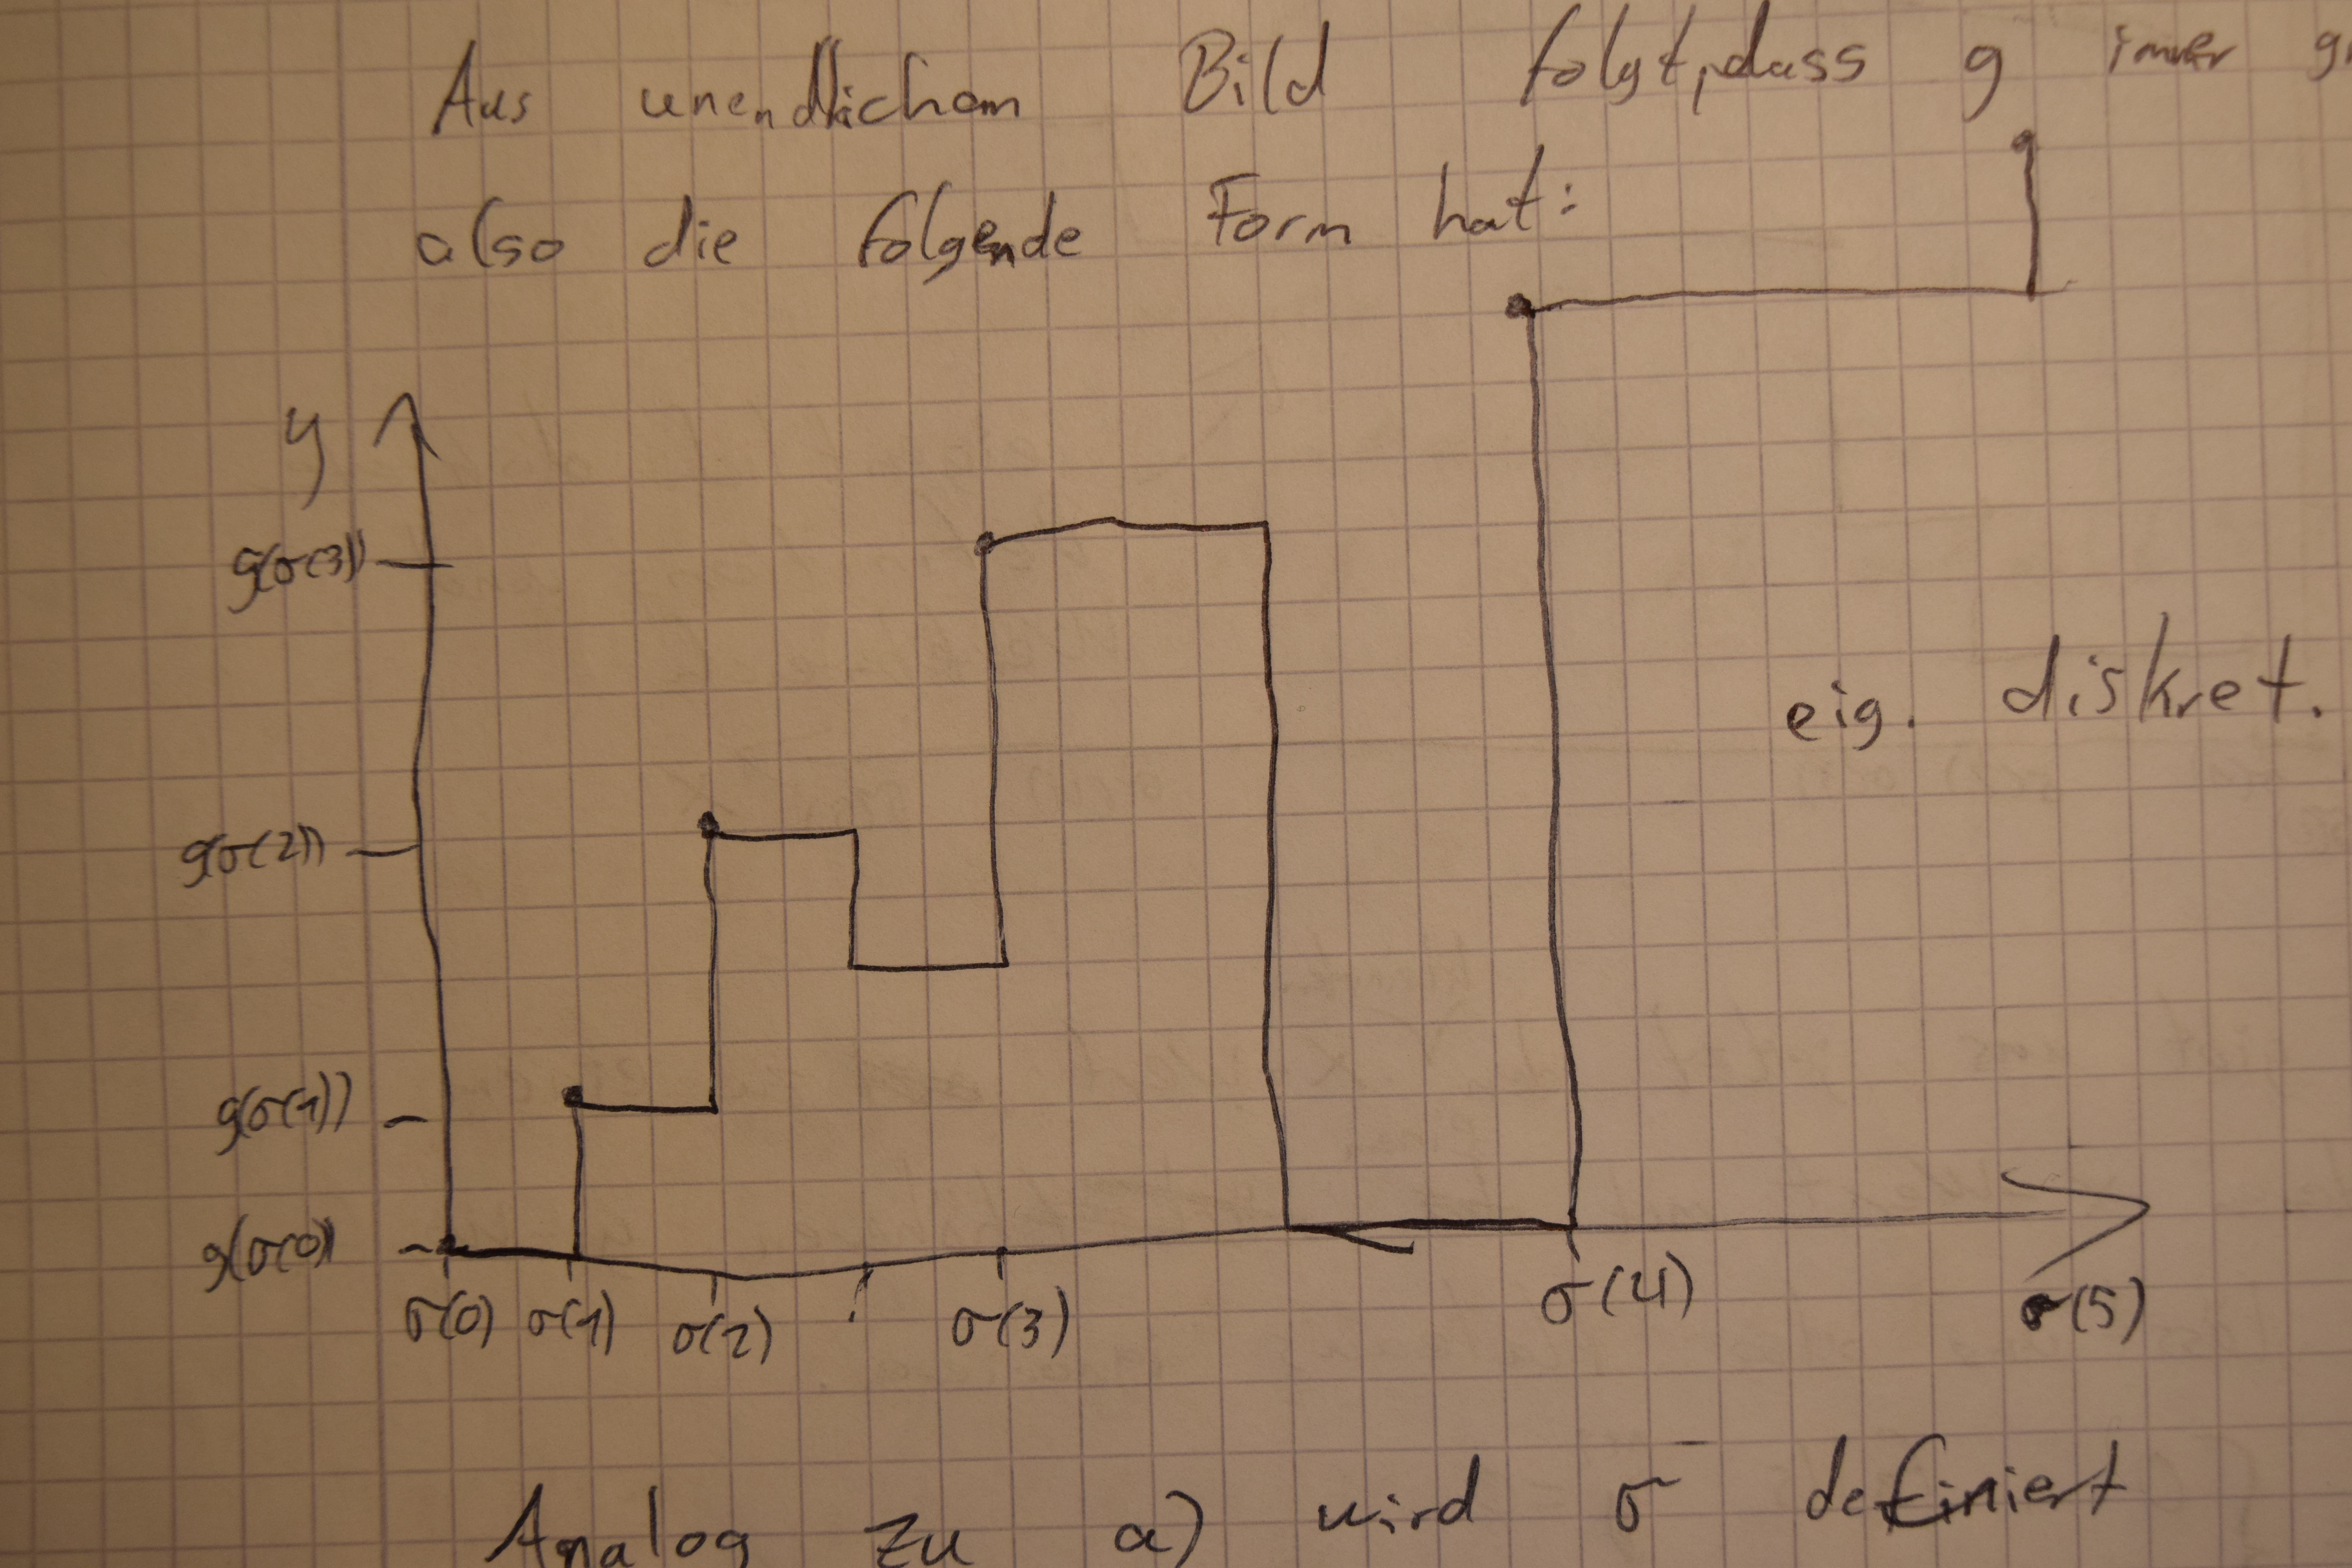
\includegraphics[scale=0.17]{./DSC_0587.JPG}
                \label{fig:./DSC_0587}
            \end{figure}
            Analog zu a) wird $\sigma$ definiert, dann ist $h = g \circ \sigma$ monoton steigend (eigentlich sogar streng monoton steigend) 
            und $h( \mathds{N}) \subset g( \mathds{N})$.\\
            \\h ist rekursiv, da $\sigma$ und g rekursiv sind.\\
        \item c)\\
            \underline{ZZ:} Jede rekursiv aufzählbare unendliche Menge $A \subset \mathds{N}$,\\
            besitzt eine rekursive unendliche Teilmenge $B \subset A$\\
            \\Nach Lemma 3.22 gibt es eine rekursive Fkt. g mit Im(g) = A\\
            $\overset{b)}{\Rightarrow}$ Es gibt ein h mit $Im(h) \subset Im(g)$, sei dann B = Im(h).\\
            Diese ist unendlich, da g unendlich ist (siehe b) und aus dem selben Grund auch rekursiv).\\
            \begin{figure}[H]
                \centering
                \includegraphics[scale=0.3]{./L-3-22.png}
                \caption{Lemma 3.22}
                \label{fig:./L-3-22}
            \end{figure}
    \end{itemize}%}}}


\section*{}
\label{sec:aufgabe_3}

    \begin{figure}[H]
        \includegraphics[scale=0.3]{./A-3.png}
        \label{fig:}
    \end{figure}

    \begin{itemize}
        \item a)\\
            $T =\\
            \{\forall x \neg x < x\} \cup \\
            \{\forall x,y,z ((x < y \land y < z) \rightarrow x <z)\} \cup \\
            \{\forall x,y (x < y \lor x \doteq y \lor y < x)\} \cup \\
            \{\forall x,y (x < y \rightarrow \exists z (x<z \land z < y))\} \cup \\
            \{\forall x \exists y (x < y)\} \cup \\
            \{\forall x \exists z (z < x)\}\\$
            \\T ist endlich und daher auch endlich axiomatisierbar.\\
        \item b)\\
            \begin{itemize}
                \item S ist nichtleer\\
                    Sei $a \in A \text{ und } b \in B$, dann ist $a \mapsto b$ in S.\\
                \item S ist Back \& Forth-System
                    \framebox{Back}\\
                    Sei F in S und $b' \in B\backslash Im(F)$\\
                    Wir unterscheiden die folgenden Fälle:\\
                    \begin{itemize}
                        \item Fall 1: $b' > F(a), \forall a \in Dom(F):\\
                            \text{Dann suche ein }a' \in A: a' > a, \forall a \in Dom(F) \text{ (Geht immer, da keine Endpunkte)}\\
                            \text{ und bilde wie folgt ab: } a' \mapsto b'$\\
                        \item Fall 2: $b' < F(a), \forall a \in Dom(F)$ ist analog.\\

\newpage

                        \item Fall 3: Sonst\\
                            Gelten die beiden Fälle, gibt es kleinere und größere Elemente als b'.\\
                            Wir wählen $a_1,a_2 \in Dom(F) \text{ so, dass gilt: } F(a_1) < b' < F(a_2)$\\
                            und $F(a_1)$ möglichst groß und $F(a_2)$ möglichst klein ist.\\
                            Dann wähle $a' \in A (=A\backslash Dom(F)): a_1 < a' < a_2$ (Geht immer, da dicht)\\
                            Und bilde $a' \mapsto b'$ ab.\\
                    \end{itemize}
                    \framebox{Forth} ist analog.\\
            \end{itemize}
            Damit sind alle Modelle elementar äquivalent $\Rightarrow$ T ist vollständig.\\
        \item c)\\
            Endlich axiomatisierbare Theorien sind rekursiv axiomatisierbar.\\
            $\overset{Korollar 3.33}{\Rightarrow}$ T ist entscheidbar, da vollständig (b)).\\

            \begin{figure}[H]
                \centering
                \includegraphics[scale=0.3]{./K-3-33.png}
                \caption{Korollar 3.33}
                \label{fig:./K-3-33}
            \end{figure}
            

    \end{itemize}

\newpage

\section*{}%{{{
\label{sec:aufgabe_4}

    \begin{figure}[H]
        \includegraphics[scale=0.3]{./A-4.png}
        \label{fig:}
    \end{figure}

    Zunächst einige Vorüberlegungen:\\
    \\A ist einfach, wenn:\\
    \begin{itemize}
        \item A rekursiv aufzählbar (nicht rekursiv!)\\
        \item $ \mathds{N}\backslash A$ unendlich\\
        \item $\nexists M \subset_{unendlich} \mathds{N} \backslash A:$ M rekursiv aufzählbar\\
    \end{itemize}
    $\Rightarrow$ A ist nicht rekursiv, sonst wäre $ \mathds{N} \backslash A$ rekursiv aufzählbar, woraus folgen würde:\\
    $M = \mathds{N} \backslash A \subset \mathds{N} \backslash A$ ist rekursiv aufzählbar \lightning\\
    \\Wir nehmen nun an, dass B rekursiv ist und führen dies zum Wiederspruch.\\
    Es gilt: $\chi_B(n) = \chi_{A\backslash \{0\}}(n+1)$\\

    \begin{itemize}
        \item Fall 1: $A = A \backslash \{0\} \Rightarrow$ A rekursiv \lightning\\
        \item Fall 2: $A = A \backslash \{0\} \cup  \{0\}$\\
            $A \backslash \{0\}, \cup \text{ und } \{0\}$ sind rekursiv.\\
            $\Rightarrow$ A ist rekursiv \lightning\\
    \end{itemize}%}}}

\end{document}
